% "{'chapitre':'dyn_1d','classe':('PSI'),'type':('application'),'titre':'Pompe à plateau', 'source':'C. Gamelon et P. Dubois','comp':('C1-05','C2-08','C2-09'),'corrige':True}"
%\setchapterimage{fig_00}
\chapter*{Application \arabic{cptApplication} \\ 
Pompe à plateau -- \ifprof Corrigé \else Sujet \fi}

\addcontentsline{toc}{section}{Application \arabic{cptApplication} : Pompe à plateau -- \ifprof Corrigé \else Sujet \fi}

\iflivret \stepcounter{cptApplication} \else
\ifprof  \stepcounter{cptApplication} \else \fi
\fi
\setcounter{question}{0}

\marginnote{D'après C. Gamelon \& P. Dubois.}
\marginnote{
\UPSTIcompetence[2]{C1-05}
\UPSTIcompetence[2]{C2-08}
\UPSTIcompetence[2]{C2-09}
}


\begin{marginfigure}
\centering
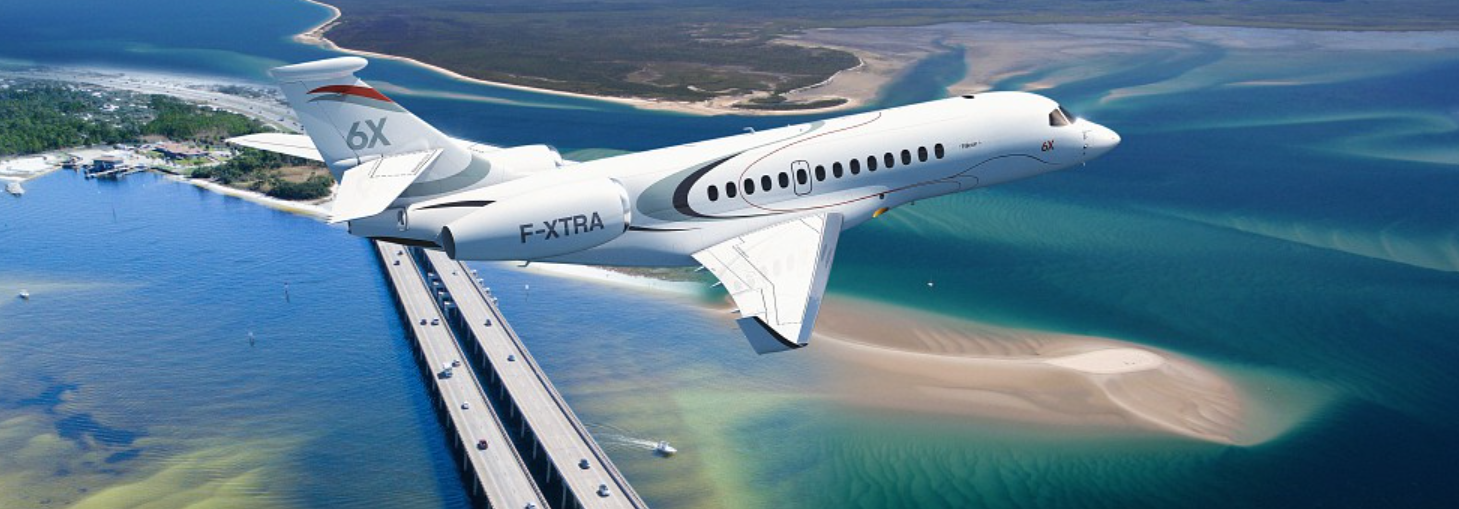
\includegraphics[width=\linewidth]{fig_00}
\end{marginfigure}


Considérons le mécanisme de pompe représenté sur la figure ci-dessous.

\begin{marginfigure}
\centering
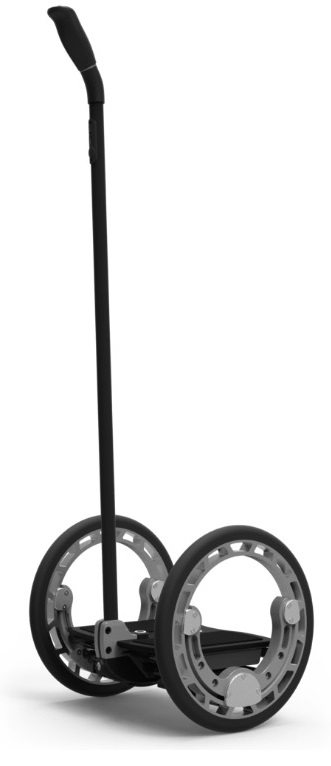
\includegraphics[width=\linewidth]{fig_01}
\end{marginfigure}

\begin{marginfigure}
\centering
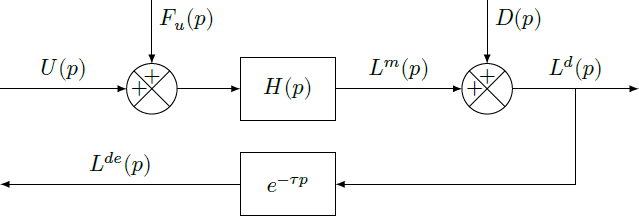
\includegraphics[width=\linewidth]{fig_02}
\end{marginfigure}


L'arbre excentrique \textbf{(1)}, animé d'un mouvement de rotation autour de l'axe $\axe{O}{x_0}$  horizontal, agit sur le piston \textbf{(2)} en liaison pivot glissant d'axe $\axe{O}{z_0}$ avec le bâti \textbf{(0)}. Pendant la phase de descente du piston \textbf{(2)}, le contact ponctuel en $I$ avec l’excentrique est maintenu par un ressort \textbf{(r)}.

\subsubsection*{Paramétrage}
Le repère $\repere{O}{x_0}{y_0}{z_0}$ lié au bâti \textbf{(0)} est supposé galiléen.
Le repère $\repere{O}{x_1}{y_1}{z_1}$ est lié à l'arbre excentrique \textbf{(1)}.
On a de plus :

\begin{itemize}
\item $\angl{y_0}{y_1}=\angl{z_0}{z_1}=\theta$;
\item $\vect{OB}=e\vect{z_1}$, $\vect{BI}=R\vect{z_0}$, $\vect{OA}=z\vect{z_0}$. 
\end{itemize} 	 	 		
 
Les liaisons pivot entre \textbf{(0)} et \textbf{(1)}, ponctuelle entre \textbf{(1)} et \textbf{(2)}, et pivot glissant entre \textbf{(0)} et \textbf{(2)} sont supposées sans frottement.
Le solide \textbf{(1)} possède un moment d’inertie $I_1$ par rapport à l'axe $\axe{O}{x_0}$. Le piston \textbf{(2)} possède une masse $m_2$.
Le ressort \textbf{(r)}, de raideur $k$, est toujours comprimé. Pour $\theta = \pm \dfrac{\pi}{2}$, l'effort de compression est égal à $\vect{F_0}=-F_0\vect{z_0}$.
Un moteur exerce un couple connu de moment $\vect{C_m}=C_m\vect{x_0}$ sur l'arbre \textbf{(1)}. Le fluide exerce sur le piston une action connue, représentée par un glisseur d'axe $\axe{O}{z_0}$ et de résultante $\vect{F_h}=-F_h{\vect{z_0}}$.

\subsubsection*{Résolution cinématique}
\question{En utilisant une fermeture géométrique ou la méthode de votre choix, déterminer la exprimer $z$ en fonction de $\theta$ et de constantes du problème. Déterminer alors $\vectv{A}{2}{0}$ et $\vectg{A}{2}{0}$.}

\subsubsection*{Résolution dynamique}

\question{Proposer une méthode permettant de déterminer l'équation différentielle du mouvement relative au paramètre $\theta$ en utilisant le PFD.}


\question{Mettre en  \oe{}uvre la méthode proposée précédemment.}

\subsubsection*{Résolution énergétique -- Pour plus tard...}
\question{Proposer une méthode permettant de déterminer l'équation différentielle du mouvement relative au paramètre $\theta$ en utilisant le théorème de l'énergie cinétique.}


\question{Mettre en  \oe{}uvre la méthode proposée précédemment.}

\subsubsection*{Pour aller plus loin...}

%\question{Avec le théorème de l'énergie cinétique, déterminer l'équation différentielle du mouvement.}

\question{En considérant un frottement sec au niveau de la liaison ponctuelle entre \textbf{(1)} et \textbf{(2)}, déterminer l'équation différentielle du mouvement.}


\ifprof
%\newpage

%TO DO : graphe de liaisons.
\textbf{Fermeture géométrique.}

On a : $\vect{OB}+\vect{BI}+\vect{IA}+\vect{AO}=\vect{0}$.

En projection sur $\vect{z_0}$ : $e\cos\theta+R=z$. Par dérivation successive, on a :
$-e\dot{\theta}\sin\theta=\dot{z}$ et $-e\ddot{\theta}\sin\theta-e\dot{\theta}^2\cos\theta=\ddot{z}$.


\textbf{On isole le solide \textbf{(1)}.}

\textbf{On réalise le bilan des actions mécaniques.}
\begin{itemize}
\item Liaison pivot : $\torseurstat{T}{0}{1}
=\torseurl{X_{01}\vect{x_0}+Y_{01}\vect{y_0}+Z_{01}\vect{z_0}}{M_{01}\vect{y_0}+N_{01}\vect{z_0}}{O}
=\torseurl{Y_{01}\vect{y_0}+Z_{01}\vect{z_0}}{\vect{0}}{O}$.
\item Liaison ponctuelle : $\torseurstat{T}{2}{1}
=\torseurl{Y_{21}\vect{y_0}+Z_{21}\vect{z_0}}{\vect{0}}{I}$. On a $Z_{21}<0$, $Y_{21}>0$ et à la limite du glissement, $Y_{21}=-fZ_{21}$. 

$\vectm{O}{2}{1}=\vectm{I}{2}{1}+\vect{OI}\wedge \vectf{2}{1}=\left( e\vect{z_1}+R\vect{z_0}\right)\wedge \left(Y_{21}\vect{y_0}+Z_{21}\vect{z_0} \right)$ 
$= -eY_{21}\cos\theta \vect{x_0}-e Z_{21}\sin\theta\vect{x_0}-RY_{21}\vect{x_0}$
$= -\left(\left(e\cos\theta+R\right)Y_{21} +e Z_{21}\sin\theta\right)\vect{x_0}$.

\item Couple moteur : $\torseurstat{T}{\text{Moteur}}{1}
=\torseurl{\vect{0}}{C_m\vect{x_0}}{O}$.
\end{itemize}

\textbf{Calcul de $\vectmd{O}{1}{0}\cdot \vect{x_0}$.}
 
$O$ est un point fixe et $I_1$ moment d'inertie par rapport à $\axe{O}{x_0}$ on a donc : 
$\vectmd{O}{1}{0}\cdot \vect{x_0}
=\left[\dfrac{\dd \vectmc{O}{1}{0}}{\dd t}\right]_{\mathcal{R}_0}\vect{x_0}
=\left[\dfrac{\dd \vectmc{O}{1}{0}\cdot \vect{x_0}}{\dd t}  \right]_{\mathcal{R}_0}$
$=\left[\dfrac{\dd \inertie{O}{1}\vecto{1}{0}\cdot \vect{x_0}}{\dd t}  \right]_{\mathcal{R}_0}$
$=\left[\dfrac{\dd I_1\dot{\theta}\vect{x_0}\cdot \vect{x_0}}{\dd t}  \right]_{\mathcal{R}_0}$
$=I_1\ddot{\theta}$.

\textbf{Application du théorème du moment dynamique en projection sur $\vect{x_0}$.}
$$
C_m-\left(\left(e\cos\theta+R\right)Y_{21} +e Z_{21}\sin\theta\right) =I_1\ddot{\theta}.
$$

\textbf{On isole le solide \textbf{(2)}.}

\textbf{On réalise le bilan des actions mécaniques.}
\begin{itemize}
\item Liaison pivot glissant: $\torseurstat{T}{0}{2}
=\torseurl{Y_{02}\vect{y_0}}{L_{02}\vect{x_0}}{O}$.
\item Liaison ponctuelle : $\torseurstat{T}{1}{2}=-\torseurstat{T}{2}{1}
=\torseurl{-Y_{21}\vect{y_0}-Z_{21}\vect{z_0}}{\vect{0}}{I}$. 
\item Ressort: $\torseurstat{T}{\text{Ressort}}{2}
=\torseurl{-F_0-kz\vect{z_0}}{\vect{0}}{A}$.
\item Pesanteur: $\torseurstat{T}{\text{Pesanteur}}{2}
=\torseurl{-m_2g\vect{z_0}}{\vect{0}}{A}$.
\item Fluide: $\torseurstat{T}{\text{Fluide}}{2}
=\torseurl{-F_h\vect{z_0}}{\vect{0}}{A}$.

\end{itemize}

\textbf{Calcul de $\vectrd{2}{0}\cdot \vect{z_0}$.}
 
$\vectrd{2}{0}\cdot \vect{z_0}=m_2\ddot{z}$

\textbf{Application du théorème de la résultante dynamique en projection sur $\vect{z_0}$.}
$$
-F_h-Z_{21}-F_0-kz-m_2g=m_2\ddot{z}.
$$


\textbf{Bilan :}
$$C_m-\left(\left(e\cos\theta+R\right)Y_{21} +e \left( -F_h-F_0-kz-m_2g-m_2\ddot{z}\right)\sin\theta\right) =I_1\ddot{\theta}.$$

On a alors :
$$C_m-\left(\left(e\cos\theta+R\right)Y_{21} -e \left( F_h+F_0+k\left( e\cos\theta+R \right)+m_2g-em_2\left( \ddot{\theta}\sin\theta+\dot{\theta}^2\cos\theta\right)\right)\sin\theta\right) =I_1\ddot{\theta}.$$


\textbf{Bilan sans frottement :}
$$C_m+e\left(
F_h+F_0+k\left( e\cos\theta+R \right)+m_2g
-em_2\sin\theta\left( \ddot{\theta}\sin\theta+\dot{\theta}^2\cos\theta\right)
\right) =I_1\ddot{\theta}.$$
\else
\fi
